\section{Appendix: Prompt Templates}
\label{appendix:prompts}

This appendix provides the complete prompt templates used in our experiments to ensure full reproducibility. All prompts are designed to enforce structured JSON output with evidence grounding.

\subsection{Category Classification Prompt}

\begin{small}
\begin{quote}
You are a strict topical classifier. Decide whether the given text is primarily about URW (Ukraine-Russia War topics) or CC (Climate Change topics).

\textbf{Rules (follow exactly):}
\begin{itemize}
\item First find the elements that indicate the topic, and reason through them step by step.
\item Output EXACTLY one label token enclosed in square brackets on the next line: \texttt{[URW]}, \texttt{[CC]}, or \texttt{[Other]}.
\end{itemize}

\textbf{Classification guidance:}
\begin{itemize}
\item Use \texttt{[URW]} for topics clearly about the Russia-Ukraine conflict.
\item Use \texttt{[CC]} for topics clearly about climate change.
\item Use \texttt{[Other]} if neither topic is the primary focus.
\end{itemize}

\textbf{Example outputs:} \texttt{EVIDENCE: short justification} followed by \texttt{[URW]}, \texttt{[CC]}, or \texttt{[Other]}.
\end{quote}
\end{small}

\subsection{Narrative Classification Prompt (Template)}

\begin{small}
\begin{quote}
You are an expert propaganda narrative analyst. Your task is to analyze the given text and identify which specific propaganda narratives are present.

\textbf{AVAILABLE NARRATIVES:}
\begin{itemize}
\item[] \{Category\}: \{Narrative Name\}
\item[] \hspace*{1em}Definition: \{Definition text\}
\item[] \hspace*{1em}Example: \{Example text\}
\item[] \hspace*{1em}Instruction: \{Instruction text\}
\end{itemize}

\textbf{INSTRUCTIONS:}

\textit{Step 1: Chain of Thought (Internal Reasoning).} Think step-by-step to analyze the text. Identify key phrases and themes. For each potential narrative, find a specific, direct quote that serves as evidence. Formulate reasoning for why that quote supports the narrative.

\textit{Step 2: Format the Final Output.} Provide a single, valid JSON object with the following schema: \texttt{\{"narratives": [\{"narrative\_name": "string", "evidence\_quote": "string", "reasoning": "string"\}]\}}
\end{quote}
\end{small}

\subsection{Sub-narrative Classification Prompt (Template)}

\begin{small}
\begin{quote}
This text is known to contain the narrative: \{Parent Narrative\}. Your task is to identify which specific sub-narratives are present.

\textbf{AVAILABLE SUBNARRATIVES:} Each sub-narrative includes its definition, example, and classification instruction. An ``Other'' option is provided for cases where the text supports the parent narrative but does not fit specific sub-narrative definitions.

\textbf{INSTRUCTIONS:}

\textit{Step 1: Chain of Thought.} Analyze the text step-by-step, looking for specific themes matching sub-narrative definitions. Find direct quotes as evidence.

\textit{Step 2: Check for Remainder.} Re-read to identify phrases supporting the parent narrative not covered by specific sub-narratives.

\textit{Step 3: Add ``Other'' if Necessary.} If uncovered evidence exists, include \texttt{\{Parent Narrative\}: Other}.

\textit{Step 4: Format Output.} Provide JSON with schema: \texttt{\{"narratives": [\{"subnarrative\_name": "string", "evidence\_quote": "string", "reasoning": "string"\}]\}}
\end{quote}
\end{small}

\subsection{Critic Validation Prompt (Narrative Level)}

\begin{small}
\begin{quote}
You are a meticulous and skeptical editor. Your task is to evaluate a classification of narratives applied to a text. You must be extremely strict. The classification is only valid if every narrative is strongly and explicitly supported by the provided evidence from the text.

\textbf{EVALUATION CRITERIA (Apply Strictly):}
\begin{enumerate}
\item \textbf{Evidence Accuracy:} Is the \texttt{evidence\_quote} an exact, verbatim quote from the original text (allowing for minor formatting differences)?
\item \textbf{Relevance of Evidence:} Does the \texttt{evidence\_quote} DIRECTLY support the \texttt{narrative\_name}? The connection must not be a stretch.
\item \textbf{Completeness:} Does the analysis miss any obvious, high-confidence narratives clearly present in the text?
\end{enumerate}

Output: Provide evaluation as a single, valid JSON object.
\end{quote}
\end{small}

\subsection{Refinement Prompt (After Critic Feedback)}

\begin{small}
\begin{quote}
You previously analyzed a text, but your analysis had flaws. A meticulous editor has provided the following feedback. Your task is to re-analyze the text, incorporating this feedback to produce a new, corrected classification.

\textbf{EDITOR'S FEEDBACK TO CORRECT:} \{Critic's feedback text\}

\textbf{ORIGINAL TASK AND DEFINITIONS:} \{Original classification prompt is repeated here\}
\end{quote}
\end{small}

\subsection{Text Cleaning Prompt}

\begin{small}
\begin{quote}
You are a precise text cleaner. Your job is to clean raw text scraped from the web by removing UI noise and boilerplate while preserving the article's content.

\textbf{STRICT RULES:}
\begin{itemize}
\item \textbf{REMOVE:} navigation menus, cookie banners, sign-up banners, button labels (e.g., `Accept', `Subscribe', `Read more'), share widgets, headers/footers, unrelated CTAs, legal disclaimers, pagination artifacts, and unrelated links.
\item \textbf{KEEP:} the main article or post content only. Preserve sentence order, punctuation, and language.
\item \textbf{DO NOT} paraphrase or summarize. Do not add or remove meaning.
\item \textbf{OUTPUT:} Return ONLY the cleaned text with no additional commentary, headings, or JSON.
\end{itemize}
\end{quote}
\end{small}

\subsection{Implementation Notes}

All prompts are implemented as Python functions that dynamically populate templates with task-specific information (e.g., available narratives, definitions, parent narrative context). The category and narrative definitions are loaded from CSV files containing the task taxonomy. This modular design allows for easy adaptation to other hierarchical multilabel classification tasks. These prompts were specifically developed and evaluated on SemEval-2025 Task 10 for multilingual narrative classification \citep{semeval2025task10}, demonstrating the generalizability of the approach across multiple languages and narrative types.

\subsection{Narrative Distribution Visualization}

\begin{figure*}[!ht]
\centering
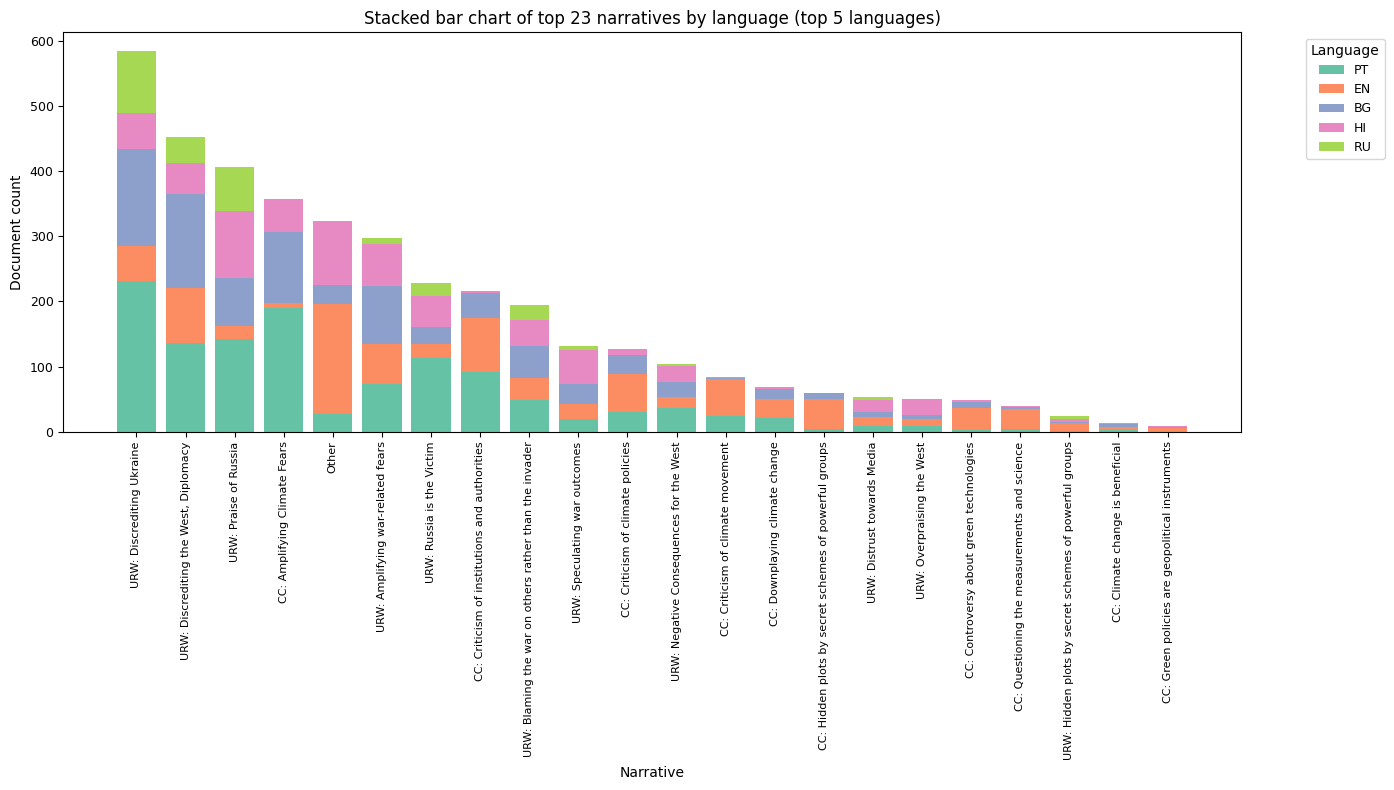
\includegraphics[width=0.95\textwidth]{assets/images/data_description/narrative_distribution.png}
\caption{Long-tailed distribution of narrative labels across the dataset. A small number of frequent narratives dominate, while most are rare. This severe imbalance (64.9:1 ratio) justifies the use of zero-shot LLM approaches that do not rely on large per-class training counts.}
\label{fig:narrative_distribution}
\end{figure*}
